\documentclass[11pt]{report}
\usepackage[a4paper, total={6in, 8.5in}]{geometry}
\usepackage{authblk}
\usepackage{graphicx}
\usepackage[section]{placeins}
\usepackage[toc,page]{appendix}
\usepackage{setspace}
\usepackage{acro}
\usepackage{textcomp}
\usepackage{multicol}
\usepackage{blindtext}
\usepackage{caption}
\usepackage[table,xcdraw]{xcolor}



\usepackage{tikz} %Charts and graphics package

\usepackage{tikzit}
\input{polarFIRstyles.tikzstyles}

\usepackage{titlepic}[cc]

\usepackage{fancyhdr} % This should be set AFTER setting up the page geometry
\pagestyle{fancy} % options: empty , plain , fancy
\renewcommand{\chaptermark}[1]{\markboth{\small\uppercase{#1}}{}}
\renewcommand{\sectionmark}[1]{}
%\renewcommand{\headrulewidth}{0pt} % customise the layout...
%\lhead{}\chead{}\rhead{}
%\lfoot{}\cfoot{\thepage}\rfoot{}
\setlength{\headheight}{14pt}

\usepackage{bytefield}

\usepackage{listings}

\usepackage{xparse}
\usepackage{amsmath}

% Graphs and plots
\usepackage{pgf,pgfplots,pgfplotstable}
\usepackage{SIunits}
%\renewcommand{\chaptername}{Part}

\pgfplotsset{compat=newest} % Allows placing the legend below the plot


% ----------  	VERILOG CODE LANGUAGE CONFIGURATION     ----------------------------------
% Adapted from https://tex.stackexchange.com/questions/377122/typesetting-for-a-verilog-lstinput
\usepackage{xcolor}
\usepackage{listings}
\definecolor{vgreen}{RGB}{104,180,104}
\definecolor{vblue}{RGB}{20, 50, 250}
\definecolor{vorange}{RGB}{255,143,102}

\lstdefinestyle{verilog-style}
{
    language=Verilog,
    basicstyle=\small\ttfamily,
    keywordstyle=\color{vblue},
    identifierstyle=\color{black},
    commentstyle=\color{vgreen},
    numbers=left,
    numberstyle=\tiny\color{black},
    numbersep=10pt,
    tabsize=8,
    moredelim=*[s][\colorIndex]{[}{]},
    literate=*{:}{:}1
}

\lstdefinestyle{c-style-old}{
  belowcaptionskip=1\baselineskip,
  breaklines=true,
  basicstyle=\small\ttfamily
  numbers=left,
  numberstyle=\tiny\color{black},
  language=C++,
  showstringspaces=false,
  basicstyle=\footnotesize\ttfamily,
  keywordstyle=\color{vblue},
  identifierstyle=\color{black},
  commentstyle=\color{vgreen},
  stringstyle=\color{orange},
  frame=single,
  xleftmargin=2em,
}

\definecolor{lbcolor}{gray}{0.95}
\definecolor{darkpurple}{hsb}{0.75, 1, 0.7}
\definecolor{darkgreen}{rgb}{0,0.4,0}

\lstdefinestyle{c-style}{
  backgroundcolor=\color{lbcolor},
  tabsize=4,
  language=C++,
  captionpos=b,
  basicstyle=\small\ttfamily,
  tabsize=3,
  frame=lines,
  numbers=left,
  numberstyle=\tiny,
  numbersep=5pt,
  breaklines=true,
  showstringspaces=false,
  identifierstyle=\color{darkpurple},
  keywordstyle=\color[rgb]{0,0,1},
  commentstyle=\color{darkgreen},
  stringstyle=\color{red}
  }
  
\lstdefinestyle{c-style-tiny}{
  backgroundcolor=\color{lbcolor},
  tabsize=4,
  language=C++,
  captionpos=b,
  basicstyle=\tiny\ttfamily,
  tabsize=3,
  frame=lines,
  numbers=left,
  numberstyle=\tiny,
  numbersep=5pt,
  breaklines=true,
  showstringspaces=false,
  identifierstyle=\color{darkpurple},
  keywordstyle=\color[rgb]{0,0,1},
  commentstyle=\color{darkgreen},
  stringstyle=\color{red}
  }

\NewDocumentCommand{\codeword}{v}{%
\texttt{\textcolor{blue}{#1}}%
}

\makeatletter
\newcommand*\@lbracket{[}
\newcommand*\@rbracket{]}
\newcommand*\@colon{:}
\newcommand*\colorIndex{%
    \edef\@temp{\the\lst@token}%
    \ifx\@temp\@lbracket \color{black}%
    \else\ifx\@temp\@rbracket \color{black}%
    \else\ifx\@temp\@colon \color{black}%
    \else \color{vorange}%
    \fi\fi\fi
}
\makeatother

\usepackage{trace}
% --------------------------END CODE DISPLAY CONFIG ----------------------------------------

%Hyperlinks:
\usepackage{hyperref}
\hypersetup{
    %bookmarks=true,         % show bookmarks bar?
    unicode=false,          % non-Latin characters in Acrobat’s bookmarks
    pdftoolbar=true,        % show Acrobat’s toolbar?
    pdfmenubar=true,        % show Acrobat’s menu?
    pdffitwindow=false,     % window fit to page when opened
    pdfstartview={FitH},    % fits the width of the page to the window
    pdftitle={FIR Filters in Vitis HLS},    % title
    pdfauthor={Alexander Stepko, axstepko.com},     % author
    pdfsubject={Implementation report},   % subject of the document
    pdfcreator={axstepko},   % creator of the document
    pdfproducer={Texifier}, % producer of the document
    pdfkeywords={}, % list of keywords
    pdfnewwindow=true,      % links in the new PDF window
    colorlinks=true,       % false: boxed links; true: colored links
    linkcolor=blue,          % color of internal links (change box color with linkbordercolor)
    citecolor=blue,        % color of links to bibliography
    filecolor=cyan,         % color of file links
    urlcolor=cyan        % color of external links
}

% -------------------------- ACRONYMS -----------------------------------------------

\DeclareAcronym{CORDIC}{
	short=CORDIC,
	long=coordinate rotation digital computer
}

\DeclareAcronym{FPGA}{
	short=FPGA,
	long=field programmable gate array
}

\DeclareAcronym{FIFO}{
	short=FIFO,
	long=first in first out
}

\DeclareAcronym{FIR}{
	short=FIR,
	long=finite impulse response
}
\DeclareAcronym{HLS}{
	short=HLS,
	long=high-level synthesis
}

\DeclareAcronym{IP}{
	short=IP,
	long=intellectual property
}

\DeclareAcronym{RTL}{
	short=RTL,
	long=register transfer level
}

\DeclareAcronym{WNS}{
	short=WNS,
	long=worst negative slack
}

% -------------------------- END ACRONYMS --------------------------------------------

%------------------------------------------------------------
%             TITLE SECTION
%------------------------------------------------------------           
\title{\Large\textbf{Design and Implementation of a Discrete FIR and CORDIC Conversion System}}
\author{Alex Stepko | \emph{axstepko.com}}

\affil{The Pennsylvania State University\\School of Electrical Engineering and Computer Science\\\normalsize{Zheyu Li, PhD. Candidate}}
\date{\today}

\titlepic{\includegraphics{media/AS_initials_blk.png}}

\renewcommand*\contentsname{Report Contents}

\fboxsep = 0mm %padding thickness
\fboxrule = 1.25pt %border thickness

\usepackage{subfiles}

\begin{document}
%\doublespacing
\begin{titlepage}
    \maketitle
\end{titlepage}
\begin{singlespace}
    \tableofcontents
\end{singlespace}
\newpage
\section*{Acronyms}
\begin{multicols}{2}
    \raggedright
    \printacronyms[heading=none]
\end{multicols}
\listoffigures
\listoftables
\lstlistoflistings
\newpage

%------------------------------------------------------------
%                 INTRODUCTION  
%------------------------------------------------------------
\chapter{Introduction}
\fancypagestyle{plain}
%% Leave some space here for the header to not place a 'T' for some reason..

This report discusses the design, optimization, and physical implementation of a complex discrete signal processing system. The processing system involves a 1-D \ac{FIR} filter in conjunction with a \ac{CORDIC} resultant in a hardware-optimized low-latency accelerator that can be used as an IP in any AXI4 compliant design. The processing chain consists of the following components:
\begin{figure}[h!]
	\centering
	\fboxsep=3mm
	\fbox{\tikzfig{FIR/polarFIRgraph}}
	\caption{Signal processing chain}
	\label{processingChainGraph}
\end{figure}

The processing chain computes a 1-D complex FIR filter on a dataset loaded to the accelerator in cartesian ($(x, y)$) format. The output of the FIR filter is also of the cartesian form. This cartesian dataset is streamed via a FIFO data channel into a CORDIC accelerator, which performs a conversion of the input vector ($(x, y)$) to the polar form ($(r, \theta)$). This data is then directed back towards the Zynq processor, which displays the product on the console.

This processing chaing was developed in Vitis HLS, an advanced \ac{HLS} synthesis tool that allows seemingly linear C (or C++/Python) code into hardware-accelerated models targeted for implementation on an \ac{FPGA}. This chain was then packaged as an \ac{IP}, and used in a block design in Vivado. Hardware was synthesized and implemented in Vivado, and the exported hardware was then used in the Vitis IDE to finish integration of the accelerator into a complete system. The target hardware for this processing chain is a Xilinx Zynq-7000 series chipset, which is held on a Digilent/Avnet/National Instruments Zedboard development board.

\vspace{1em}

\colorbox{red!15}{\parbox{\linewidth}{\noindent\textbf{Note to Developers:} All source code for this project can be found on the \href{https://github.com/FPGACrashCourse/ComplexFIRFilter}{GitHub repository} (\href{https://github.com/FPGACrashCourse/ComplexFIRFilter}{https://github.com/FPGACrashCourse/ComplexFIRFilter}).}}

\section{Processing chain}
\subsection{FIR filter}\label{FIRtheory}

The FIR filter is a fundamental technique used in countless systems in the medical, defense, academic, and consumer sectors. Moreover, a high-performance FIR filter is almost always necessary in a signal processing chain. Generically, the formula for a complex FIR filter is
\begin{equation}
    Y = \sum_{i=0}^{n}w_i * X[n - i]
\end{equation}
for any arbitrary set of inputs. This is equivalent to a 1-D convolution. This can be extended to complex vectors, which results in an almost identical equation of the form
\begin{equation}
	\overline{Y} = \sum_{i=0}^{n} w_i * \overline{X}[n-i]
\end{equation}
where $\overline{Y}$, $w_i$, and $\overline{X}[n-i]$ are of the general complex form $\overline{Z} = \alpha + j \beta$ (in cartesian coordinates). While this result is desierable in most scenarios, a more useful form of the result exists in polar form, where generically the same vector can be represented as $\overline{Z} = (r, \theta)$ in polar coordinates. In standard trigonometry, this conversion is trivial. For the rectangular vector $\overline{Z} = \alpha + j \beta$, we find its polar form with the following equations
\begin{equation}
	r = \sqrt{\alpha^2 + \beta^2}
\end{equation}
\begin{equation}
	\theta = \tan^{-1}\left({\frac{\beta}{\alpha}}\right)
\end{equation}
which results in the vector $\overline{Z} = (r, \theta)$. While the average individual can quickly compute these values with a calculator, the computational power required to reach these results is rather large. In a setting where realtime performance is necessary, these calculations are nearly impossible to achieve or require an unreasonably large amount of compute power.

\subsection{CORDIC}\label{cordicTheory}

A well-known method to perform trigonometry and coordinate system conversion is the \ac{CORDIC}. This system iteratively rotates a vector using simple matrix multiplication to the desired target, and then applies a simple gain factor. Because it is multiplication on a base-two numerical system, it is possible to achieve this with a simple right-shift and addition/subtraction of the vector to rotate. The generic form for a CORDIC rotation is

\begin{equation}
\begin{bmatrix}
\cos \theta & -\sin \theta \\
\sin \theta & \cos \theta \\
\end{bmatrix}\begin{bmatrix}
x_{i-1} \\
y_{i-1} \\
\end{bmatrix}
= \begin{bmatrix}
x_i \\
y_i \\
\end{bmatrix} 
\end{equation}
which is resultant in
\begin{equation}\label{CORDICxCalc}
x_i = x_{i-1}  \cos \theta - y_{i-1}  \sin \theta\
\end{equation} and 
\begin{equation}\label{CORDICyCalc}
y_i = x_{i-1} \sin \theta + y_{i-1} \cos \theta\
\end{equation}
being the rotated versions of the original vector $[x_{i-1}, y_{i-1}]$. This algorithm is iterative, and therefore it rotates by decrementing amounts towards the target angle. While the rotation correctly computes to the raw angle, it fails to correctly compute the converted magnitude. This is easily fixed by a single multiplication of the CORDIC gain factor. Gain factors are computed iteratively with the equation
\begin{equation}\label{gainEQ}
K(n) = \prod_{i=0}^{n-1} K_i  = \prod_{i=0}^{n-1}\frac {1}{\sqrt{1 + 2^{-2i}}}
\end{equation} and  
\begin{equation}
K = \lim_{n \to \infty}K(n) \approx 0.6072529350088812561694
\end{equation}
which are normally computed and stored in a lookup table for quick-reference without computing the result in realtime. 

\begin{table}
\begin{center}
\begin{tabular}{|c|c|c|c|c|c|}
\hline
i & $2^{-i}$ 	& Rotating Angle  	& Scaling Factor 	& CORDIC Gain 	\\ \hline \hline
0 & 1.0 		& $45.000^{\circ}$	& 1.41421			& 1.41421		\\ \hline
1 & 0.5 		& $26.565^{\circ}$	& 1.11803			& 1.58114		\\ \hline
2 & 0.25 		& $14.036^{\circ}$	& 1.03078			& 1.62980		\\ \hline
3 & 0.125 		& $7.125^{\circ}$	& 1.00778			& 1.64248		\\ \hline
4 & 0.0625 	& $3.576^{\circ}$	& 1.00195			& 1.64569		\\ \hline
5 & 0.03125 	& $1.790^{\circ}$	& 1.00049			& 1.64649		\\ \hline
6 & 0.015625 	& $0.895^{\circ}$	& 1.00012			& 1.64669		\\ \hline
\end{tabular}
\end{center}
\caption{CORDIC gains for the first six iterations of the algorithm}
\label{table:cordic}
\end{table}
\FloatBarrier

As noticed above, the CORDIC gain $K_i$ increases with each iteration. If we compute $K_i ^{-1}$, we then see that the gain decreases as iterations increase. This fact is only important in the sense that after a certain point of iterations, the gains are practically identical until the $10^{-9}$ decimal point. Essentially, beyond a certain number of iterations the precision of the algorithm plateaus at almost the exact correct value.




%%%%%%%%%%%%%%%%%%%%%%%%%%%%%%%%%%

\subfile{FIR/FIR.tex}

\subfile{CORDIC/CORDIC.tex}

\chapter{Complete Processing Chain}

The complete processing chain consists of the FIR filter and CORDIC cartesian-to-polar converter shown in Figure \ref{processingChainGraph}. Systems which may employ such a chain commonly include real-time audio processing, wireless communication, medical imaging, and radar systems - to name a few.  

The internal architecture of the complete processing chain is rather simple, it serves as a top-level I/O handler for the chain, and handles data between processing elements. Data is transferred between the FIR filter and CORDIC via \codeword{HLS::stream} objects. These objects act as a \ac{FIFO} queue between functions to ensure efficient single-element data transfer without substantial read/write delays. The syntax to declare datastreams between the two chain elements is shown in Listing \ref{streamSyntax}

        \begin{singlespace}
            \lstinputlisting[breaklines=true,
            label={streamSyntax},
            caption={Stream syntactical use},
            style=c-style,
            language=C++,
            firstnumber=81,
            linerange={81-90},]{../source/polarFIR.cpp}
        \end{singlespace}

Additonally, the complete processing chain uses the appropriate precompiler directives to set the AXI4-compliant interface for the device. Particularly, the usage of a memory-access interface is desired (set/get various data with driver functions). This enables export as a Xilinx IP, and its subsequent use in a Vivado product. An example of the interface is shown in Listing \ref{interfaceSyntax}

        \begin{singlespace}
            \lstinputlisting[breaklines=true,
            label={interfaceSyntax},
            caption={AXI4 interface declaration},
            style=c-style,
            language=C++,
            firstnumber=60,
            linerange={60-68},]{../source/polarFIR.cpp}
        \end{singlespace}
        
The resultant top-level function completes the processing chain developed in the HLS environment. No optimization is performed in this top-level function (aside from the \codeword{HLS::stream}s), as it is unnecessary given the granular development of the component processsing stages.

\section{Hardware development}\label{hwPackage}

This HLS product was exported as a fully AXI4-compliant interface IP for usage in a Vivado design. This IP allows transport between different hardware targets, and also protects any sensitive processing trade-secrets from being made public. 

This HLS IP was brought into a Vivado block diagram. Additionally, the Zynq processing system and the necessary AXI4 protocol systems was connected using the connection automation function in Vivado. The complete block diagram for the system is seen below in Figure \ref{fig:BD}.

\begin{figure}[h!]
 	\begin{center}
 		\fboxsep=0mm
 		\fbox{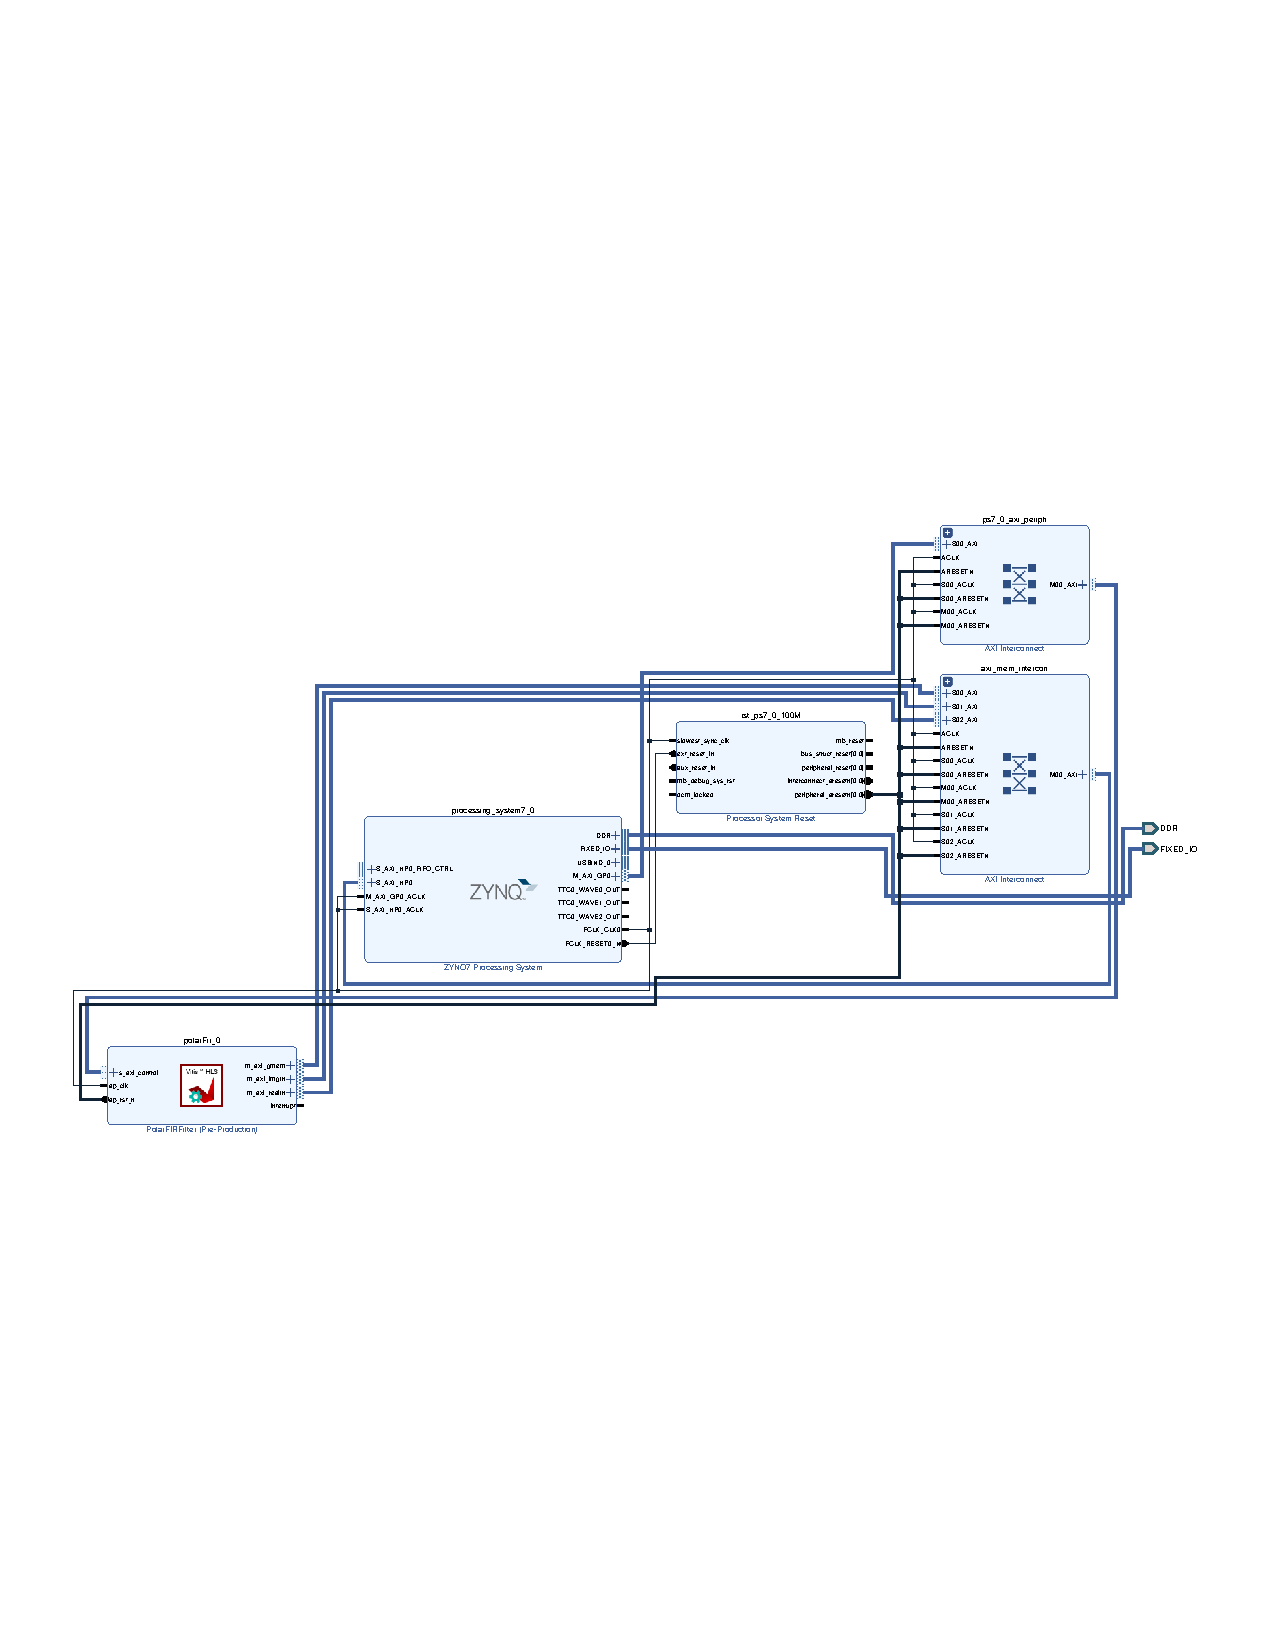
\includegraphics[width=\textwidth]{media/blockDesign.pdf}}
 		\caption{Hardware block diagram}
 		\label{fig:BD}
 	\end{center}
 \end{figure}
 \FloatBarrier
 
 The block diagram provides further abstraction from the source code written in C++ (and the Verilog products), and lets the deployment process happen much more quickly. The block diagram was then wrapped, and a RTL diagram was generated. The design was then synthesized implemented, and packaged as a \texttt{.xsa} file for usage in Vitis IDE as a development platform. 
 
 \begin{figure}[h!]
 	\begin{center}
 		\fboxsep=0mm
 		\fbox{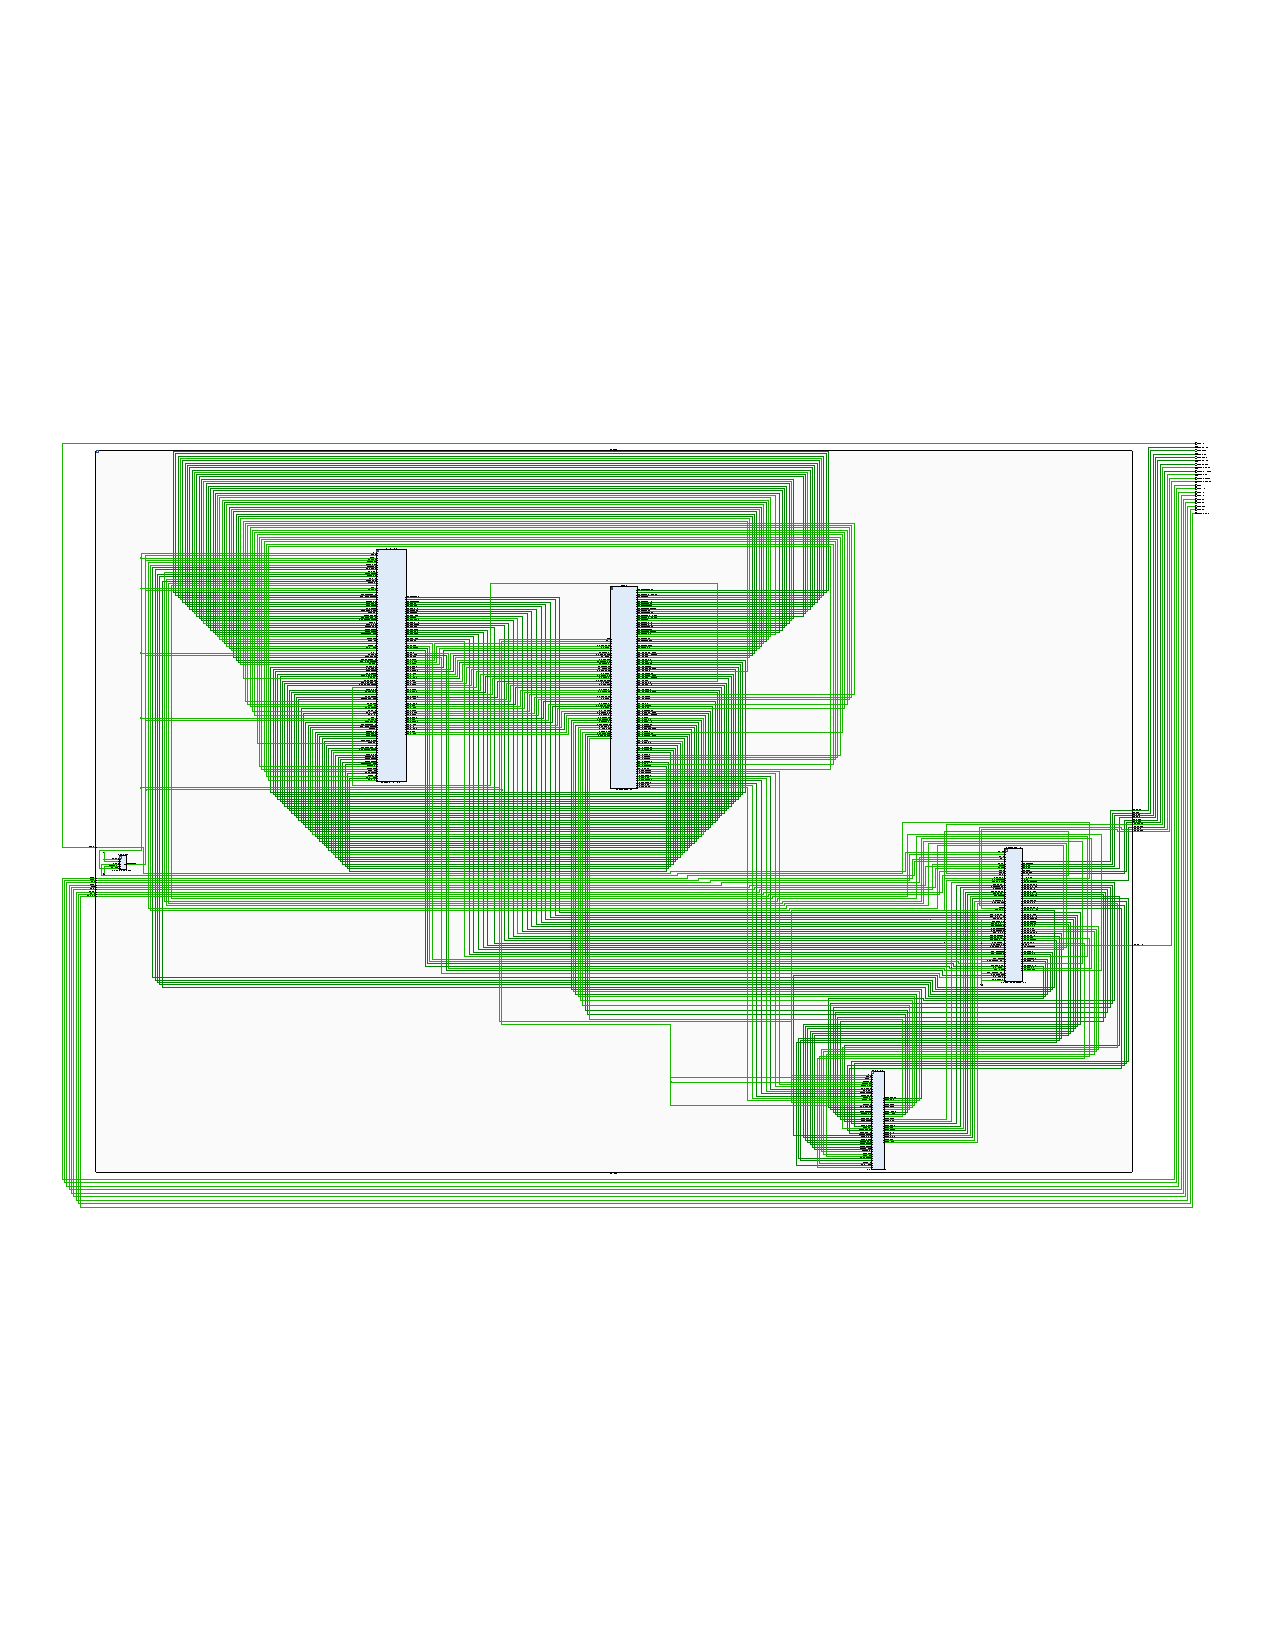
\includegraphics[width=\textwidth]{media/schematic.pdf}}
 		\caption{RTL schematic}
 		\label{fig:RTL}
 	\end{center}
 \end{figure}
 \FloatBarrier
 

\section{Vitis IDE interaction development}

The hardware design created in section \ref{hwPackage} was brought into Vitis IDE as the last step in the development stack to generate a functional product. In the IDE, we develop an interaction function to initiate, start, and obtain results from any given processing chain.

In addition to the hardware design, Vitis HLS provides a set of driver functions for utilization of a HLS product in a complete system. These functions are necessary to interact with the HLS IP. The generated drivers include typical hardware interaction functions, such as set/get of data, initialization, start/stop, and status returns. The function declarations are included in Listing \ref{xpolarfirDeclarations}, although the specifics don't essentially matter.

What is crucially important is that the order-of-operations is followed to initialize the hardware to its proper state before running the accelerator. This is accomplished with a set of functions provided in the driver, but is abstracted slightly for ease-of-development. The source code for this abstraction layer is provided in Listing \ref{IPcontrolSource}.

With a functional driver, it is possible to interact with the accelerator and validate its functionality. This is accomplished via a top-level application, who's source code can be found in Listing \ref{mainIDEsource}.

The high-level functionality of the source code is to generate an input and filter set, run the accelerator, and print out the results. Data fed into the filter is a \codeword{u32} datatype, and is memory-mapped to pointers shown below in Listing \ref{mainDatamap}

	   \begin{singlespace}
            \lstinputlisting[breaklines=true,
            label={mainDatamap},
            caption={Primary datatypes},
            style=c-style,
            language=C++,
            firstnumber=120,
            linerange={120-128},]{../IDE/polarFIR_r10/src/main.c}
        \end{singlespace} 
        
Then, with the datatypes properly generated and allocated, the accelerator is set with that data. Additionally, the output products of the system are mapped, as shown in Listing \ref{mainIOmap}.

	   \begin{singlespace}
            \lstinputlisting[breaklines=true,
            label={mainIOmap},
            caption={Main application source code},
            style=c-style,
            language=C++,
            firstnumber=137,
            linerange={137-141},]{../IDE/polarFIR_r10/src/main.c}
        \end{singlespace} 
        
Once this process is complete, we run the accelerator using the \codeword{runHardware();} function provided by the IP-control abstraction layer.
        
 
\section{Validation}
       
Validation of the hardware's functionality in the IDE is rather simple. Because the components were tested in HLS, the final validation is to check if the IDE product can properly interact with the accelerator. This is accomplishe via running the hardware (as previously mentioned), and then waiting for the hardware to return it has finished computation. 

With the final results, we print the output results. Using a test dataset of the input vectors, filter coefficents, we initialize the dataset and run the test. We obtain the following output from the IDE after running the accelerator:


\begin{figure}[h!]
 	\begin{center}
 		\fboxsep=0mm
 		\fbox{\includegraphics[width=0.2\textwidth]{media/IDEterminalInput.png}}
 		\caption{Input dataset}
 		\label{fig:inputResults}
 	\end{center}
 \end{figure}
 \FloatBarrier
 
\begin{figure}[h!]
 	\begin{center}
 		\fboxsep=0mm
 		\fbox{\includegraphics[width=0.5\textwidth]{media/IDEterminalOutput.png}}
 		\caption{Output data}
 		\label{fig:outputResults}
 	\end{center}
 \end{figure}
 \FloatBarrier
 
 Manual calculation of these results verifies that the FIR filter correctly performs a filter pass, and the CORDIC computes the output value of the system. We consider the design to be complete, and have conducted a thorough study of its performance. 
 
 Future work on this processing system look to allow interaction of the design using other data inputs aside from fixed numbers. Using audio or downconverted RF samples provides the basis for a rudementary processing system capable of detecting phase changes in a given signal. Additionally, the high-throughput of the design ensures that processing latency is kept to a minimum, and hardware resources are also minimized.
     
        %%%%%%%%%%%%%%%%%%%%%%%%%%%%%%%%%%%%%%%%%%%%%%%%%%%%%%%%%%%

\begin{appendices}
    \chapter{Top-level processing chain source code}
        \begin{singlespace}
            \lstinputlisting[breaklines=true,
            label={TOPheader},
            caption={Top-level processor code (header)},
            style=c-style,
            language=C++,
            firstnumber=1,]{../source/polarFIR.h}
        \end{singlespace}

        \begin{singlespace}
            \lstinputlisting[breaklines=true,
            label={TOPsource},
            caption={Top-level processor code},
            style=c-style,
            language=C++,
            firstnumber=1,]{../source/polarFIR.cpp}
        \end{singlespace}

	\chapter{Cartesian FIR Filter code}
        \begin{singlespace}
            \lstinputlisting[breaklines=true,
            label={FIRsourceheader},
            caption={Cartesian FIR filter source code (header)},
            style=c-style,
            language=C++,
            firstnumber=1,]{../source/complexFIR.h}
        \end{singlespace}

        \begin{singlespace}
            \lstinputlisting[breaklines=true,
            label={FIRsource},
            caption={Cartesian FIR filter source code},
            style=c-style,
            language=C++,
            firstnumber=1,]{../source/complexFIR.cpp}
        \end{singlespace}
        
    \chapter{CORDIC source code}
        \begin{singlespace}
            \lstinputlisting[breaklines=true,
            label={CORDICsource},
            caption={CORDIC source code (header)},
            style=c-style,
            language=C++,
            firstnumber=1,]{../source/CORDIC.h}
        \end{singlespace}   
        
        \begin{singlespace}
            \lstinputlisting[breaklines=true,
            label={CORDICsource},
            caption={CORDIC source code},
            style=c-style,
            language=C++,
            firstnumber=1,]{../source/CORDIC.cpp}
        \end{singlespace}
       
     \chapter{Custom datatype source code}
        \begin{singlespace}
            \lstinputlisting[breaklines=true,
            label={datatypeHeader},
            caption={CORDIC source code},
            style=c-style,
            language=C++,
            firstnumber=1,]{../source/datatypes.h}
        \end{singlespace} 
        
        \chapter{Vitis IDE source code}   
        
         \begin{singlespace}
            \lstinputlisting[breaklines=true,
            label={mainIDEsource},
            caption={Main application source code},
            style=c-style,
            language=C++,
            firstnumber=1,]{../IDE/polarFIR_r10/src/main.c}
        \end{singlespace} 
        
      \chapter{Hardware accelerator source code}
        \begin{singlespace}
            \lstinputlisting[breaklines=true,
            label={ValidationSource},
            caption={Hardware validation source code},
            style=c-style,
            language=C++,
            firstnumber=1,]{../source/hwValidation.cpp}
        \end{singlespace} 
   
        \chapter{Hardware driver source code}
                \begin{singlespace}
            \lstinputlisting[breaklines=true,
            label={xpolarfirDeclarations},
            caption={HLS-generated driver declarations},
            style=c-style,
            language=C++,
            firstnumber=1,]{hwSrc/xpolarfir.h}
        \end{singlespace} 
        
        \begin{singlespace}
            \lstinputlisting[breaklines=true,
            label={IPcontrolHeader},
            caption={Driver interaction function (header)},
            style=c-style,
            language=C++,
            firstnumber=1,]{../IDE/polarFIR_r10/src/IPcontrol.h}
        \end{singlespace} 
        
         \begin{singlespace}
            \lstinputlisting[breaklines=true,
            label={IPcontrolSource},
            caption={Driver interaction function},
            style=c-style,
            language=C++,
            firstnumber=1,]{../IDE/polarFIR_r10/src/IPcontrol.c}
        \end{singlespace} 
        
        
        
        

\end{appendices}


\end{document}



























